\part{Introduction}

\lecture{\centerline{\Large Syllabus: Organisation and Course Introduction}}{semaine 1}

\section{Organisation}

\subsection{Syllabus}
\begin{frame} \frametitle{Syllabus}
  \begin{tabular}[c]{lrl}
    Week   & Date  & \\\hline
    Week 2 & 7/01  & Course/TP\\
    Week 3 & 14/01 & Course/TP\\
    Week 4 & 21/01 & Course/TP\\
    Week 5 & 28/01 & Course/TP\\
    Week 6 & 04/02  & Course/Projects\\
    Week 7 & 11/02 & Course/Projects\\
    Week 8 & 18/02 & \alert{Vacations}\\
    Week 9 & 25/01 & Course/Projects\\
    Week 10 &03/03 & Course/Projects\\
  \end{tabular}
  \begin{block}{}
    \begin{itemize}
    \item 8 courses sessions (duration: 1.5h)
    \item 4 exercise sessions (duration: 1.5h)
    \item 4 homework/projects sessions (duration: 1.5h)
    \end{itemize}
    
  \end{block}

\end{frame}

\begin{frame} \frametitle{Horaires des Cours/TPs}
  \begin{itemize}
  \item Les cours auront lieu en F211 de 8:00 � 9:30 
  \item les TP et Projets auront lieu
    \begin{itemize}
    \item en F212 de 17:00 � 18:30 les semaines 2,3,4,5
    \item en F218 de 8:00 �   9:30 les semaines 5,6,7,9,10
    \end{itemize}
  \end{itemize}
\end{frame}


\begin{frame} \frametitle{Note Finale}
  \begin{itemize}
  \item $N_p$ note projet(environ 10 minutes de pr�sentation et 5 minutes de questions)
  \item $N_e$ note examen
  \item $N_{\mathrm{TP}}$ note TP 
  \item La participation sur l'ensemble du cours permettra d'augmenter la note finale
  \item $N$ note finale
  \end{itemize}
  \begin{alertblock}{Note Finale}
  \[ N = \min ( .5 N_p + .3 N_e +  .2 N_{\mathrm{TP}}+ \mathrm{participation}, 20) \]    
  \end{alertblock}


\end{frame}

\subsection{Notes de Cours, TP et Projets}
\begin{frame}{Notes de Cours, TP et Projets}

  \begin{block}{}
    \begin{itemize}
    \item Les notes de cours, les TP et projets seront disponibles sur
      le Bureau Virtuel Rhones Alpes (� partir du 15 Janvier)
    \item Les notes de cours seront disponibles apr�s que le cours ait
      �t� donn�
    \item Une liste de projets sera disponible courant Janvier
    \item Les TP doivent �tre rendus la veille du cours au plus tard � minuit 
    \end{itemize}
  \end{block}

\end{frame}

\begin{frame}{Quelques Id�es de Projets}
  \begin{block}{}
    
    \begin{itemize}
    \item Simulation d'une syst�me de refroidissement pour un
      micro-processeur
    \item Simulation d'un micro-onde en 2D et 3D
    \item Multigrille parall�le avec Trilinos
    \end{itemize}
    \alert{Vous pouvez �galement proposer des sujets }
  \end{block}
\end{frame}

\subsection{}
\begin{frame}{Questions?}
  \centerline{Questions?}
\end{frame}

\subsection{Definition and Position}

\begin{frame}<1-2>{Scientific Computing: Definition}

      \only<1>{
        \begin{block}{What is Scientific Computing?}
        Can someone give a definition?
      \end{block}
      }
      \only<2>{
        \begin{block}{What is Scientific Computing?}
        Everything that is related to computing in science
      \end{block}        
      \begin{example}
        Geophysics, Astrophysics, Weather forecast, Global Change,
        Plasma physics, Aerodynamics, Hydrodynamics, MHD, Rheology,
        Materials processing, Molten metals, Finance 
      \end{example}
    }

\end{frame}

\begin{frame}{Scientific Computing: Position}

  \begin{block}{Position}
      How would you position Scientific Computing?
  \end{block}

\end{frame}

\begin{frame}
  \frametitle{Scientific Computing~(S.C.) = $\cap $\{Math.,Comp.Sci,Model.\}}
  \begin{columns}
    \begin{column}{.6\textwidth}
      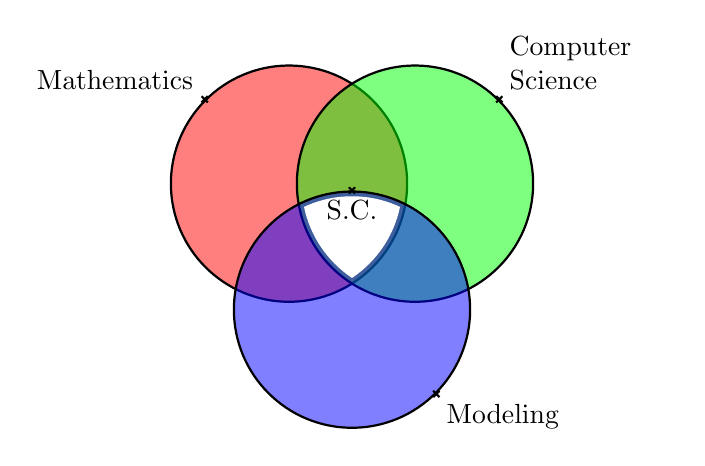
\begin{tikzpicture}[thick, scale=.8]
        \draw (0,2) node[fill=red,fill opacity=0.5,draw,shape=circle,name=cs,minimum size=3cm] {};
        \draw (2,2) node[fill=green,fill opacity=0.5,draw,shape=circle,name=math,minimum size=3cm] {};
        \draw (1,0) node[fill=blue,fill opacity=0.5,draw,shape=circle,name=model,minimum size=3cm] {};
        
         \begin{scope}{fill=white,fill opacity=1}
           \clip (0,2) circle (1.8cm);
           \clip (2,2) circle (1.8cm);
           \clip (1,0) circle (1.8cm);
           \fill[white] (1,0) circle (3cm);
         \end{scope}
         write label
         \draw[shift=(cs.north west)] plot[mark=x] coordinates{(0,0)} node[anchor=north east,text width=2cm,text ragged,above left] {Mathematics};
         \draw[shift=(math.north east)] plot[mark=x] coordinates{(0,0)} node[anchor=north west,text width=2cm,text ragged,above right] {Computer Science};
         \draw[shift=(model.south east)] plot[mark=x] coordinates{(0,0)} node[anchor=south west,text width=2cm,text ragged,below right] {Modeling};
         \draw[shift=(model.north)] plot[mark=x] coordinates{(0,0)} node[below] {S.C.};
      \end{tikzpicture}
    \end{column}
    \begin{column}{.4\textwidth}
      \begin{itemize}
      \item Primary objective:\\
        Mumerical experiments

      \item Secondary objective:\\
        \alert{How} to obtain them
        \begin{itemize}
        \item Mathematics
        \item Computer science/Software design
        \end{itemize}
      \end{itemize}
    \end{column}
  \end{columns}
  \begin{alertblock}{Richard Hamming}
    The purpose of computing is insight, not numbers
  \end{alertblock}
\end{frame}


\begin{frame}
  \frametitle{Domains of SC}

  \begin{block}{Some Domains}
  \begin{itemize}
  \item Military
  \item Basic research
  \item Industry
  \item Economy
  \item Life Sciences
  \end{itemize}
  \end{block}
\end{frame}


\begin{frame}
  \frametitle{Goals of SC}
  \begin{block}{Some Goals}
    \begin{itemize}
    \item Improvement of technological design (Airplanes, Cars, Ships)
    \item Improving security (Car crash simulations)
    \item Advanced methodologies (Molting, Burning)
    \item Understanding of physical phenomena (Big bang, Astrophysics)
    \item Design/interpretation of experiments (Plasma physics, High energy physics)
    \item More efficient production and higher quality (Tissue cutting)
    \item Forecasts (Weather, Bourse, Climate)
    \item Comparisons (Data base search, Web, Genomics, Proteomics)
    \item Recognition, detection (Image processing)
    \item Constant evaluation (business, statistics)
    \end{itemize}
  \end{block}

\end{frame}


\begin{frame}
  \frametitle{Numerical Simulation Cycle}

  \tikzstyle{root concept}+=[concept color=white!80]
  \tikzstyle{level 1 concept}+=[concept color=red!80, sibling angle=72]
  \tikzstyle{every annotation}=[fill=black!50,opacity=0.5,text=white,scale=.7]
  \begin{tikzpicture}[->]
     \path[mindmap,concept color=black!60,text=white]
     node[concept,scale=.7] {Numerical Simulation Cycle}
     %node[concept,scale=.7] {Scientific Computing}
     [clockwise from=0]
     %child[concept,scale=.6] { node[concept,scale=.7] (phys) {Physics Mechanics Biology Processing} }
     child[concept,scale=.6] { node[concept,scale=.7] (phys) {Modeling} }
     child[concept,scale=.6] { node[concept,scale=.7] (am) {Applied   Math.} }
     child[concept,scale=.6] { node[concept,scale=.7] (nm) {Numerical   Math.} }
     child[concept,scale=.6] { node[concept,scale=.7] (cs) {Computer Science} }
     child[concept,scale=.6] { node[concept,scale=.7] (va) {Validation} }
     ;
     \node [annotation,right] at (phys.south east)
     {
       \begin{itemize}
       \item Geophysics
       \item Astrophysics
       \item Weather forecast
       \item Global Change
       \item Plasma physics
       \item Aerodynamics
       \item Hydrodynamics
       \item MHD
       \item Rheology
       \item Materials processing
       \item Molten metals
       \item Finance
       \end{itemize}
     };
     \node [annotation,right] at (am.south east)
     {
       \begin{itemize}
       \item Statistics
       \item Functional Analysis
       \item Partial differential equations,
       \item Stochastic equations, etc.
       \end{itemize}
     };
     \node [annotation,left] at (nm.south west)
    {
      \begin{itemize}
      \item Numerical Analysis:
        Convergence, Errors
      \item Approximation methods:
        Space/time discretization
        FD, FE, FV, spectral
        method, particle
        simulation
      \item Algorithms: complexity, accuracy
      \item Mesh Generation, CAD
      \item Direct / iterative solvers
      \end{itemize}
    };
    \node [annotation,left] at (cs.south west)
    {
    \begin{itemize}
    \item Architecture: vector, parallel,  scalar, cluster.
    \item Systems, Compilers. Libraries
      \item Data management, Visualisation
      \item Parallelisation: MPI, OpenMP
      \item Optimisation, Parameterisation
      \end{itemize}
    };
    \node [annotation,right] at (va.east)
    {
      \begin{itemize}
      \item Interpretation of numerical experiment
      \item Comparison with experiment

      \item \alert{Correction of models}
      \end{itemize}
    }
    ;

    \begin{pgfonlayer}{background}
      \draw [concept connection]
      (phys) edge node[above,sloped]{Analyze} (am)
      (am) edge node[above,sloped]{Analyze} (nm)
      (nm) edge node[above,sloped]{Implement} (cs)
      (cs) edge node[above,sloped]{Run} (va)
      (va) edge node[above,sloped]{Correct} (phys);
     \end{pgfonlayer}

\end{tikzpicture}
\end{frame}


\subsection{Scientific Computing History}
\subsubsection{Hardware}

\begin{frame}
  \frametitle{Pioneers}
  \begin{tabular}[c]{clll}
   1642	& Blaise Pascal	& Mechanical & 	Add, substract for tax collection\\

   1820	& C. F. Gauss & Human &		Least square fits (geodesy)\\

   ~1850 & Charles Babbage & Difference engine & Add, substract, multiply, divide\\
         &                  &  Programmable    & Ada Lovelace	\\
    
   ~1935 & Konrad Zuse	& EM relays		& Destroyed 1944 \\
    
   1943	& Alan Turing &	Tubes, relays 	& Colossus (code breaking computer)\\

   1946	& Eckert/Mauchley &	Tubes, relays	& Eniac -> Univac\\

   1948	& John von Neumann &	Tubes &		IAS (modern serial architecture)\\

   1948	& Bardeen, Brattain, Shockley&&		Transistor invention\\

   1972	& Slotnick, Burroughs, & NASA	&	Illiac IV (array processor)\\

   1975 &	Seymour Cray	& Cray 1&		Vector computer
    
  \end{tabular}
\end{frame}
\begin{frame}
  \frametitle{Pioneers}
  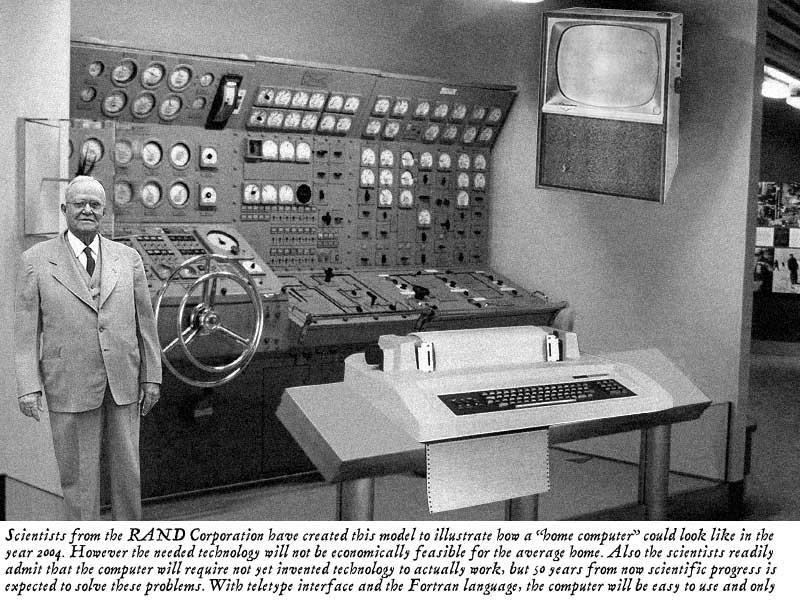
\includegraphics[width=.85\textwidth]{computer_pioneer}
\end{frame}

\begin{frame}{Computer Generations}
  \begin{tabular}[c]{clll}
    First & 1945-54 & Vacuum tubes &	Mark 1, ENIAC, IAS, IBM 701\\

    Second &	1955-64 & Transistors	& CDC 1604, IBM 7000\\

    Third &	1965-74 & Integrated circuits &	CDC 6600\\

    Fourth &	1975-90	& LSI/VLSI &		Cray 1, VAX 9000\\

    Fifth &	1991-now & ULSI/VHSIC &	Cray T3D, Intel Paragon\\
  \end{tabular}
\end{frame}

\subsubsection{Software }

\begin{frame}{Software History}
  
  \begin{tabular}[c]{lcl}
    Ada Lovelace	& 1850 &		Programmable difference scheme \\
    Konrad Zuse		& 1945 &		Plankalk�l (algorithmic language)\\
    Grace Hopper	& 1954 &		Flowmatic (first compiler)\\
    John Backus		& 1955 &		Fortran\\
    Bauer/Rutishauser	& 1958 &		Algol\\
    Task Force		& 1959 &		Cobol\\
    K.E. Iverson	& 1962 &		APL (first parallel language)\\
    D. Richie		& 1972 &		C\\
    Richie, Thompson	& 1978 &		Unix\\
    Niklaus Wirth	& 1978 &		Modula-2 (OOP)\\
    J. Ichbiah		& 1979 &		ADA\\
    B. Stroustrup	& 1983 &		C++\\
    Linus Thorvald	& 1992 &		Linux\\
    V.S. Sundaram	& 1990 &		PVM\\
    MPI Forum		& 1995 &		MPI\\
    Sun			& 1995 &		Java\\

  \end{tabular}
  
\end{frame}
\subsubsection{Algorithms}
\begin{frame}{Algorithms History}
  \begin{tabular}[c]{lcl}
    Pythagoras, Thales	& -5th &		Geometry\\
    Al-Khwarizmi	& 900 &		Algorithms\\
    Persia/Irak		& 1000 &		Algebra\\
    Jobst B�rgi		& 1610 &		Logarithms\\
    John Napier		& 1614 &		Natural logarithms\\
    J.B.J. Fourier	& 1808 &		Fourier Transform\\
    C.F. Gauss		& 1820 &		Gauss elimination/Least squares\\
    C.G.J. Jacobi	& 1845 &		Jacobi method\\
    R. Courant		& 1943 &		Finite elements\\
    Ulam, Metropolis	& 1946 &		Monte Carlo\\
    C. Lanczos		& 1950 &		Lanczos method\\
    Stiefel, Hestenes	& 1952 &		Conjugate gradients\\
    H. Rutishauser	& 1958 &		LR/QR\\
%    B.J. Alder		& 1959 &		Molecular dynamics\\
    G.B. Dantzig	& 1963 &		Linear programming\\
    Cooley, Tukey	& 1965 &		FFT\\
    A. Brandt		& 1973 &		Multigrid\\
%    Car, Parinello	& 1985 &		Car Parinello method\\
  \end{tabular}
\end{frame}

\subsection{A Few Quotes}
\begin{frame}{A Few Quotes}
  \begin{block}{John von Neumann (Dec 28, 1903 - Feb 8, 1957)}
    It would appear that we have reached the limits of what it is
    possible to achieve with computer technology, although one should
    be careful with such statements, as they tend to sound pretty silly
    in 5 years. 
  \end{block}
\end{frame}

\begin{frame}{Quotes}
  \begin{block}{Edsger W. Dijkstra (1930-2002)}
%% When we had no computers, we had no programming problem
%% either. When we had a few computers, we had a mild programming
%% problem. Confronted with machines a million times as powerful, we
%% are faced with a gigantic programming problem.

    \begin{enumerate}
    \item  Besides a mathematical inclination, an exceptionally good mastery
      of one's native tongue is the most vital asset of a competent
      programmer.
      
    \item Programming is one of the most difficult branches of applied
      mathematics; the poorer mathematicians had better remain pure
      mathematicians.
      
    \end{enumerate}
    
  \end{block}
\end{frame}
%% Edsger W. Dijkstra (1930-2002) was a Dutch Computer Scientist,
%% invented the concept of "structured programming".
%%\end{frame}

\subsection{Objectives of the Course}
\begin{frame}
  \frametitle{What is this course about ?}
  \begin{block}{Learning about}
    \begin{itemize}
    \item Scientific programming environments
      \begin{itemize}
      \item Compilers (C/C++)
      \item Scientific Libraries
      \item Programs for scientific computing
      \end{itemize}
    \item Scientific programming
    \item Pre and post processing
    \end{itemize}
  \end{block}
  \begin{alertblock}{What if Scenarii}
    Imagine a situation where you don't have any commercial software
    to solve a given scientific computing problem:
    \centerline{What would you do ?}
  \end{alertblock}
\end{frame}

\begin{frame}<1-7>{What Would You Do?}
  \begin{block}{}
  \begin{itemize}[<+-| alert@+>]
  \item Ask the person that seem to know a lot about computing in your company
  \item Ask Google
  \item Ask other search engines
  \item Ask FOSS Community
  \item Ask your preferred GNU/Linux / FreeBSD distro  
  \item What else ?
  \end{itemize}
    
  \end{block}
  \only<7>{
    \begin{alertblock}{FOSS}
      We shall use FOSS
    \end{alertblock}
  }
\end{frame}

\subsection{Scientific Computing Programs}
\begin{frame}[label=scprog]
  \frametitle{What does a scientific program look like?}

  \tikzstyle{root concept}+=[concept color=gray!60]
  \tikzstyle{level 1 concept}+=[concept color=red!80, sibling angle=180]
  \tikzstyle{every annotation}=[fill=black!50,opacity=0.5,text=white,scale=.8]
  \begin{tikzpicture}[->]
    \path[mindmap,concept color=gray!70,text=white]
    node[concept,scale=.7] (proc) {Processing}
    % node[concept,scale=.7] {Scientific Computing}
    [clockwise from=0]
    % child[concept,scale=.6] { node[concept,scale=.7] (phys) {Physics Mechanics Biology Processing} }
    child[concept,scale=.7] { node[concept,scale=.7] (post) {Post Processing} }
    child[concept,scale=.7] { node[concept,scale=.7] (pre) {Pre Processing} }
    ;
    \node [annotation] at (proc.south)
    {
      \begin{itemize}
      \item Approximation methods: Space time discretisation, FE, FV,
        Particle methods,...
      \item Linear Algebra
      \end{itemize}
    };
    \node [annotation] at (pre.south)
    {
      \begin{itemize}
      \item Computer Aided Design (CAD)
      \item Mesh generation
      \end{itemize}
    };
    \node [annotation] at (post.south)
    {
      \begin{itemize}
      \item Interpretation of results
      \item Visualisation
      \end{itemize}
    };

    \begin{pgfonlayer}{background}
      \draw [concept connection,->]
      (pre) .. controls +(up:2cm) and +(up:2cm) .. node[above,sloped] {Data Handling} (proc)
      (proc) .. controls +(up:2cm) and +(up:2cm) .. node[above,sloped] {Data Handling} (post);
     \end{pgfonlayer}

  \end{tikzpicture}
\end{frame}

\begin{frame}
  \frametitle{Pre-Processing}
  \begin{block}{}
    \begin{itemize}
    \item CAD (OpenCascade)
    \item Mesh generation (gmsh, netgen, tetgen, ...)
    \item Data acquisition, properties(material...), ...
    \end{itemize}
  \end{block}
\end{frame}
\begin{frame}
  \frametitle{Processing: Algorithmic methodologies}
  \begin{block}{}
  \begin{itemize}
  \item Global functions approximations (FFT, wavelets, spectral methods)
  \item Local functions approximations (FE, FV, FD, p method)
  \item Monte Carlo simulations (MD, LB)
  \item Particle pushing (Gyrotron, Granular flow)
  \item Ray tracing (Image processing)
  \item Sequencing (Genomics, proteomics)
  \item Data handling (DB, Web)\\[.5cm]

  \item Direct solvers
  \item Iterative solvers
  \item Time evolution (implicit, explicit)
  \item Eigenvalue problems
  \end{itemize}
  \end{block}
\end{frame}
\begin{frame}
  \frametitle{Processing: Parallel methods}
  \begin{block}{}
    \begin{itemize}
    \item Domain decomposition method
    \item Local parallelism (Point-to-point: FE, FV, FD, p-method)
    \item Global parallelism (All-to-many: FFT, wavelets, spectral)
    \item Redistribution/equilibration (Particle pushing)
    \item Embarassingly parallel applications (Master/slave: DB,
      Web, sequencing, ray tracing, parameter studies, statistics)
    \end{itemize}
  \end{block}
\end{frame}

\begin{frame}{PostProcessing}
  \begin{block}{}
    \begin{itemize}
    \item Visualisation (Paraview, Octave, Pyx, Matplotlib,...)
    \item Analysis, validation
    \item Archive (HDF5,...)
    \item Error estimation, Adaptation, go back to preprocessing
    \end{itemize}
  \end{block}
\end{frame}


\begin{frame}
  \frametitle{Software aspects}
  \begin{block}{A few things to consider}
    \begin{itemize}
    \item Control if results are correct: Bugs, not applicable models
    \item Improve precision: Single/double, stability (CFL), h,p,r methods
    \item Numerical experiments: Validation of models, interpretation of results
    \item Choose stable methods
    \item Convergence properties
    \item Portability, extensibility
    \item Efficiency, scalability, choice of adequate machine
    \item Engineering time: Production cycle, GUI
    \item Implementation aspects
    \end{itemize}
  \end{block}
\end{frame}



\begin{frame}
  \frametitle{Some words of wisdom?}
  \begin{block}{Machines}
    \begin{itemize}
    \item Use best single processor algorithms
    \item Parallelise, but only if single processor version is too slow/small
    \end{itemize}
  \end{block}
  \begin{block}{Applications/algorithms}
    \begin{itemize}
    \item Use what exists
    \item Use libraries, since they are efficiently implemented
    \end{itemize}
  \end{block}
\end{frame}


%%% Local Variables: 
%%% mode: latex
%%% TeX-master: "scicomp"
%%% TeX-PDF-mode: t
%%% TeX-parse-self: t
%%% x-symbol-8bits: nil
%%% TeX-auto-regexp-list: TeX-auto-full-regexp-list
%%% ispell-local-dictionary: "american"
%%% End: 


